%%
%INTERPOLATING SCHEDULES
%%

\begin{figure}[!ht]
  \centering
  \subfloat[][original Roland-Cerf s(t)]
  {
    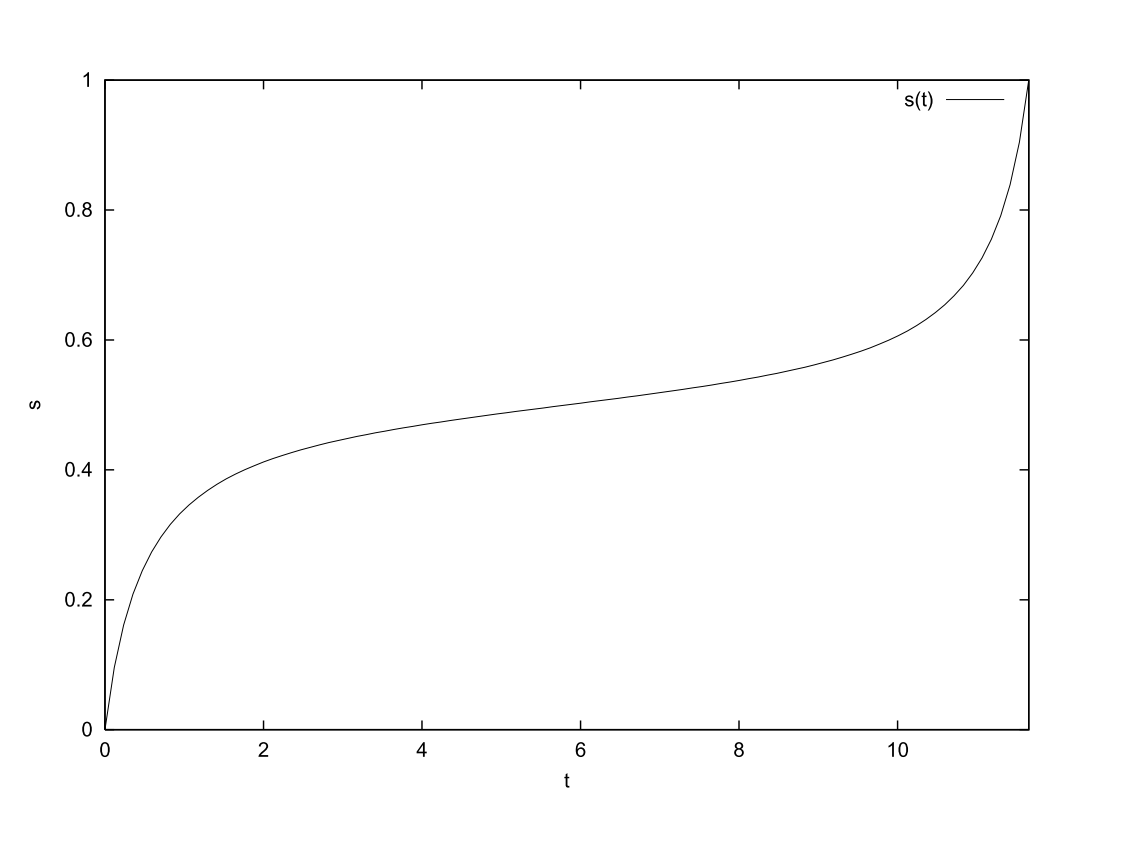
\includegraphics[width=50mm]{./figures/interpolating_schedules/cerf}
  }

  \subfloat[][our $s_{RC}(t)$]
  {
  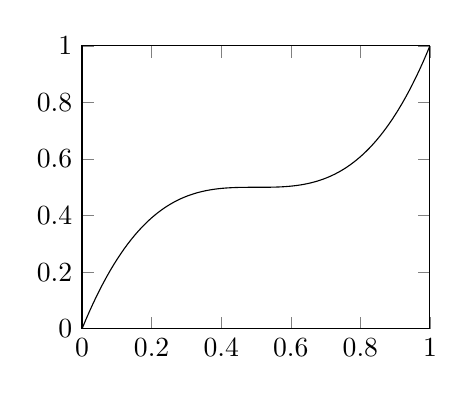
\begin{tikzpicture}
    \begin{axis}[name=plot,
    domain=0:1, restrict y to domain=0:1,
    xmin=0, xmax=1,
    ymin=0, ymax=1,
    width = 60mm,
    samples=100
    ]

    \addplot[color=black]{(0.5)*((2*x-1)^3+1)};

    \end{axis}
  \end{tikzpicture}
  }


  \caption{\textbf{Roland and Cerf's interpolating schedule (a) and our Roland-Cerf like schedule (b).} These figures show the difference between the original interpolating schedule derived by Roland and Cerf for the unstructured search (left) and our $s_{RC}(t)$(right). Although quite different we study the effects of this particular non-linear interpolating schedule and compare it with the linear one used by Farhi and Gutmann \cite{Farhi2000}.}
  \label{fig:interpolating_schedule_compared}
\end{figure}
